\part{Conjoncture et politiques économiques} % (fold)
\label{prt:conjoncture_et_politiques_economiques}

Les différents organismes économiques, réalisent des prévisions de taux de croissance du PIB. Mais leurs prévisions divergent de part les modèles utilisés et 
les hypothèses réalisées.

L'approche macroéconomique de ce chapitre, se base sur l'analyse de keynes et la synthèse néoclassique ensuite opérée. On étudiera les modèles IS-LM. En effet 
l'économiste Kaldor, propose d'analyser les phénomènes macro à l'aide du "carré magique".

\begin{figure}[h]
	\begin{center}
		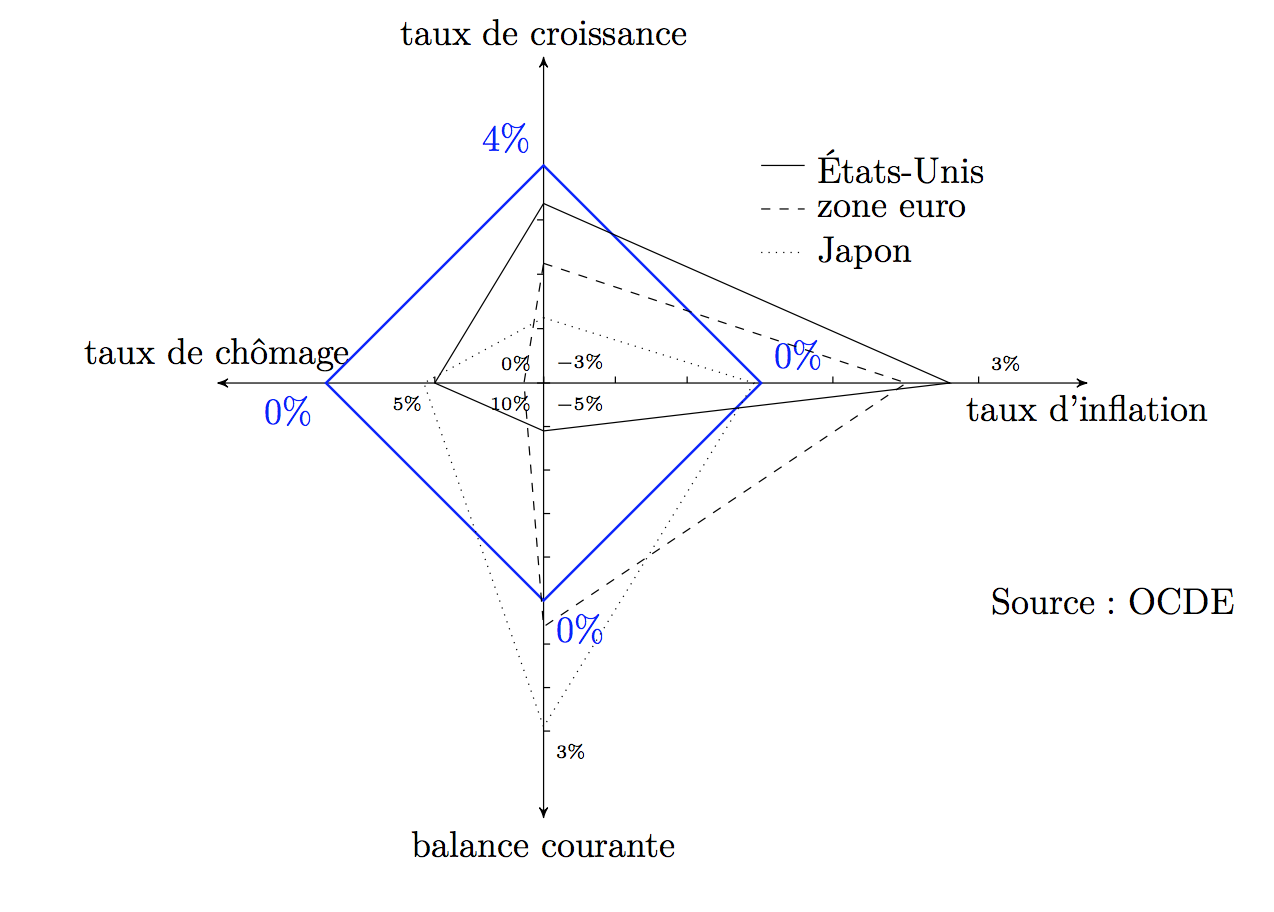
\includegraphics[scale=0.5]{./img/im2}
		\caption{"Carré magique": moyénné de 1996 à 2006}
	\end{center}
\end{figure}

Les différents axes du "carré magique" reprèsentent les objectifs de la politique macroéconomique. On s'ntéressera dans ce chapitre aux 3 premiers. On recueille
différentes politiques économiques, chronologiquement discernables comme il suit : 
\begin{itemize}[label=\ding{69}]
	\item \emph{Les trente glorieuses (45-73)}: une politique plus simple. Une réponse parfaite à l'analyse keynésienne, en cas de récession et chômage élevé
	on instaurait des politques budgétaires et monétaires expansionistes (le contraire si chômage faible et inflation). On parle de politique de \textsc{Stop and Go}, la représentaiton économique de ce phénomène s'appelle \emph{la courbe de Phillips}.
	\item 
\end{itemize}

% part conjoncture_et_politiques_economiques (end)